\section*{Cíle laboratorního cvičení}
\begin{itemize}
  \item Seznámení se se signalizačním protokolem SIP.
  \item Peer-to-peer VoIP pomocí signalizace SIP.
  \item Komunikace VoIP pomocí signalizace SIP přes ústřednu.
\end{itemize}

\section*{Základní instrukce}
\begin{itemize}
  \item Pro práci ve cvičení budete používat následující virtuální stroje v programu VirtualBox:
  \begin{itemize}
	\item \textbf{PC-A}: První klient (Jitsi).\\
	Virtuální stroj: \url{https://nes.fit.vutbr.cz/isa/ISA2020.ova}
	\begin{table}[H]
		\centering
		\begin{tabular}{|c|c|}
		\hline
		\textbf{Uživatelské jméno} & \textbf{Heslo} \\ \hline
		root                       & root4lab       \\ \hline
		user                       & user4lab       \\ \hline
		\end{tabular}
	\end{table}

	\item \textbf{PC-B}: Druhý klient (Jitsi).\\
	Virtuální stroj: PC-B vytvoříte v průběhu laboratoře klonováním PC-A dle návodu níže.
	\begin{table}[H]
		\centering
		\begin{tabular}{|c|c|}
		\hline
		\textbf{Uživatelské jméno} & \textbf{Heslo} \\ \hline
		root                       & root4lab       \\ \hline
		user                       & user4lab       \\ \hline
		\end{tabular}
	\end{table}
	\item \textbf{PC-U}: Ústředna (Asterisk).\\
	Virtuální stroj: \url{http://nes.fit.vutbr.cz/isa/isa-asterisk.ova}
	\begin{table}[H]
		\centering
		\begin{tabular}{|c|c|}
		\hline
		\textbf{Uživatelské jméno} & \textbf{Heslo} \\ \hline
		root                       & root       \\ \hline
		isa                       & isa       \\ \hline
		\end{tabular}
	\end{table}
  \end{itemize}
  \item Pokud z předchozích cvičení máte provedeny nějaké změny ve virtuálních strojích, obnovte je do výchozího stavu.
  \item Před zahájením cvičení si vytvořte snapshot virtuálního stroje za pomoci
  menu \textit{Machine $\rightarrow$ Take snapshot} pro snadný návrat k výchozímu stavu.
  \item Odpovědi pište do odpovědního archu \texttt{protokol.md} který odevzdáte do WIS-u.
  Dostupný je na adrese \url{https://github.com/nesfit/ISA/blob/master/voip/protokol.md}.
  \item Do WIS-u budete také odevzdávat všechny zachycené \texttt{pcap} soubory.
\end{itemize}

\section{Instalace Jitsi SoftPhone na PC-A}
\begin{itemize}
  \item Jitsi SoftPhone je aplikace, která simuluje chování fyzického IP telefonu.
  
  \item Pro instalaci Jitsi SoftPhone na CentOS 7 je nejdříve potřeba vyřešit problém se závislostmi na požadované RPM balíčky. Na PC-A zadejte postupně následující příkazy:\footnote{Zdroj: \url{https://github.com/jitsi/jitsi/issues/425#issuecomment-345938823}}
      
	\begin{verbatim}
	rpm -e --nodeps speex
	
	wget https://copr-be.cloud.fedoraproject.org/results/fedpop/speex/
	epel-7-x86_64/00146973-speex/speex-1.2-0.23.rc2.el7.centos.x86_64.rpm
	
	rpm -i speex-1.2-0.23.rc2.el7.centos.x86_64.rpm
	
	wget https://copr-be.cloud.fedoraproject.org/results/fedpop/speexdsp/
	epel-7-x86_64/00146970-speexdsp/speexdsp-1.2-0.7.rc3.el7.centos.x86_64.rpm
	
	rpm -i speexdsp-1.2-0.7.rc3.el7.centos.x86_64.rpm
	\end{verbatim}
	
  \item Následně spusťte lokální instalaci Jitsi SoftPhone na PC-A příkazem
  
  \verb{yum localinstall https://github.com/jitsi/jitsi/releases/download/Jitsi-2.10/{\\
  \verb{jitsi-2.10-5550.x86_64.rpm{
  
  \item V případě problémů se stažením RPM balíčku z oficiálního zdroje, můžete zkusit instalaci z alternativního zdroje příkazem\\
  \verb{yum localinstall http://rover.borec.cz/jitsi-2.10-5550.x86_64.rpm{
  
  \item Pokud instalace selže (např. chyba související s Python), obnovte virtuální stroj do výchozího stavu (ze snímku vytvořeného před začátkem laboratoře) a pokuste se o instalaci Jitsi ještě jednou.
\end{itemize}

\section{Peer-to-peer VoIP pomocí signalizace SIP}
Se svým sousedem nastavte komunikaci VoIP mezi Vašimi dvěma počítači bez použití ústředny (spojení peer-to-peer).

\begin{enumerate}
    \item Zapněte program Jitsi a vyčkejte až se spustí okno programu.
    \item V menu {\bf Options} $\rightarrow$ {\bf Accounts} přidejte nový účet. Pro ten nastavte pole {\bf Network} na hodnotu {\bf SIP} a následně {\bf SIP id} na hodnotu 10XX, kde {\bf XX je číslo Vašeho počítače}, potvrďte tlačítkem {\it Add} a zkontrolujte, že se vytvořil {\it RegistrarLess SIP} účet.
    \item Spusťte síťový analyzátor Wireshark a začněte zachytávat pakety na rozhraní, kterým jste připojeni k síti.
    \item Po spuštění nastavte display filtr tak, aby zobrazoval pouze protokol
      SIP (Display Filter: sip).
    \item V hlavním okně programu zadejte do pole {\it Enter name or number} SIP adresu Vašeho souseda: \linebreak{\bf 10.10.10.1YY}, kde {\bf YY} je číslo počítače Vašeho souseda.
    \item Zavolejte Vašemu sousedovi stisknutím zeleného telefonu. Na druhém počítači přijměte hovor, vyzkoušejte, zda se se sousedem navzájem slyšíte a po chvíli hovor ukončete.
(V případě problémů se zvukem zkontrolujte, zda není v systému ztlumen mikrofon, či audio výstup, případně v aplikaci Jitsi v menu Options $\rightarrow$ Audio zkontrolujte nastavení zvukových zařízení.) 
    \item Proveďte analýzu navazování spojení v odchycených datech ve Wiresharku. Využijte podpory v menu {\bf Telephony $\rightarrow$ VoIP Calls}, kde uvidíte jednotlivé zaznamenané hovory. Vyberte příslušný hovor a pro zobrazení průběhu klikněte na volbu {\bf Flow}.
    \item Zakreslete spojení do grafu v protokolu. Uveďte, pomocí kterých protokolů a mezi jakými IP adresami a porty probíhá signalizace a přenos dat. Zjistěte použitý kodek pro přenos hlasu.
\end{enumerate}
Názvy a čísla podporovaných kodeků lze zobrazit v SIP/SDP zprávě v sekci {\bf Session Initiation Protocol} $\rightarrow$ {\bf Message body} $\rightarrow$ {\bf Session description protocol}:
\begin{figure}[h!]
  \centering
  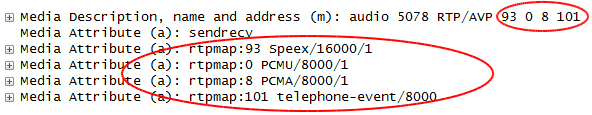
\includegraphics[width=145mm]{img/3a.png}
\end{figure}

\noindent Informace o tom, který z podporovaných kodeků byl skutečně použit získáte z RTP paketů (Filter: RTP) podle čísla v poli {\bf Payload type}.
\begin{figure}[h!]
  \centering
  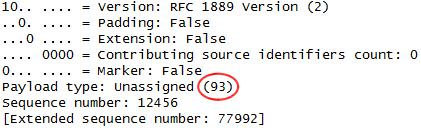
\includegraphics[width=105mm]{img/3b.png}
\end{figure}


\section{Komunikace VoIP pomocí signalizace SIP přes ústřednu}
Se svým sousedem nastavte komunikaci VoIP mezi vašimi dvěma počítači pomocí SIP ústředny umístěné v laboratorní síti.

\subsection{Analýza registrace a odregistrace}
\begin{enumerate}
    \item Spusťte znovu zachytávání paketů v aplikaci Wireshark tlačítkem 
\includegraphics[width=3mm]{img/ws_start.png}.
    \item Vraťte se do hlavního okna aplikace Jitsi, otevřite menu {\bf Options} $\rightarrow$ {\bf Accounts}.
    \item Vytvořte nový účet, v poli {\bf Network} vyberte hodnotu SIP, přepněte se do rozšířených nastavení (tlačítkem {\bf Advanced}) a postupujte podle obrázků \ref{fig:sip_account} a \ref{fig:sip_connection}, kde místo {\bf XX}, dosaďte číslo Vašeho počítače.\\
\begin{figure}[h!]
  \centering
  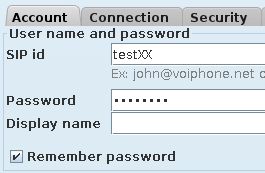
\includegraphics[scale=0.8]{img/sip_account.png}
  \caption{Základní informace o účtu.}
  \label{fig:sip_account}
\end{figure}
\begin{figure}[h!]
  \centering
  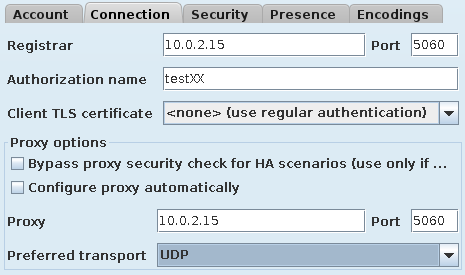
\includegraphics[scale=0.8]{img/sip_connection.png}
  \caption{Informace o připojení, přihlašovací jméno k ústředně a proxy.}
  \label{fig:sip_connection}
\end{figure}
    a potvrďte tlačítkama {\bf Next $\rightarrow$ Sign in}.
    \item Tímto jste provedli registraci k ústředně. Pokud jste vše nastavili správně, mělo by se v pravém sloupci zobrazit {\bf SIP Online} \\
    {\it (V případě neúspěchu v nastavení účet odeberte a znovu přidejte. Pokud ani toto nepomohlo, ukončete Jitsi a postupujte znovu od kroku 1), případně konzultujte problém se cvičícím}
    \item V menu {\bf Options} $\rightarrow$ {\bf Accounts} vytvořený SIP účet a klikněte na {\bf Delete}, čímž by měla proběhnout odregistrace od ústředny.
    \item Ve Wiresharku analyzujte registraci a odregistraci a zakresleslete jejich průběh do protokolu. Vyplňte požadované údaje a zjistěte, v čem se liší paket, kterým se registrujete, od paketu, kterým se odregistrujete.
\end{enumerate}


\subsection{Analýza hovoru přes ústřednu}
\begin{enumerate}
    \item Znovu se registrujte k ústředně stejně jako v předchozí sekci.
    \item Obnovte zachytávání paketů v aplikaci Wireshark tlačítkem 
\includegraphics[width=3mm]{img/ws_start.png}.
    \item V hlavním okně programu zadejte do pole pro telefonní číslo/adresu SIP adresu Vašeho souseda: \linebreak{\bf 10YY@10.10.10.222}, kde {\bf YY} je opět číslo počítače Vašeho souseda.
    \item Zavolejte Vašemu sousedovi a proveďte analýzu hovoru podobně jako u Peer-to-peer hovoru.
    \item Zakreslete průběh spojení do grafu v protokolu. Zkombinujte informace
      z obou pracovních stanic a do protokolu zaneste úplnou komunikaci všech
      tří stanic. Uveďte, mezi kterými IP adresami a porty probíhá signalizace a mezi kterými přenos dat. Vyplňte, které protokoly se používají pro signalizaci a které pro přenos. Dále zjistěte, jaký kodek pro přenos hlasu byl použit.
\end{enumerate}

\section{Ukončení práce v laboratoři}
\begin{itemize}
  \item Počítač vypněte spuštěním (jako {\bf root}) skriptu {\tt /root/isa4/clean}.
\end{itemize}
